\documentclass[a4paper,12pt]{report}
\usepackage[spanish,mexico]{babel}
\usepackage[utf8]{inputenc}
\usepackage[T1]{fontenc}
\usepackage{amsmath}
\usepackage{amssymb}
\usepackage{wasysym}
\usepackage[dvipsnames,pdftex]{color}
\usepackage[x11names]{xcolor}
\usepackage{tikz, tkz-euclide}
\usepackage[american]{circuitikz}
\usepackage{siunitx}
\usetikzlibrary{arrows}
\usepackage[colorinlistoftodos]{todonotes}
%\usepackage[left=2cm,right=1.5cm,top=1cm,bottom=1cm]{geometry}
%\usepackage{helvet}
%\renewcommand{\familydefault}{\sfdefault}
\setlength{\oddsidemargin}{0in}
\usepackage{geometry}
\geometry{a4paper, total = {180mm,270mm},
			left = 25mm, top = 20mm,
            right=15mm,bottom=20mm,%
            footskip=10mm}
\usepackage{float} 
% \setlength{\topmargin}{0in}
% \setlength{\voffset}{-0.5in}
% \setlength{\hoffset}{0.3in}
% \setlength{\textheight}{700pt}
% \setlength{\textwidth}{440pt}
% \setlength{\topskip}{0in}
% \setlength{\parskip}{2ex}
 \renewcommand{\baselinestretch}{1.5}
\usepackage{diagbox}
\usepackage{array}
\usepackage{listings}
\usepackage{caption}
%%% comandos definidos por el usuario
\begin{document}
\setcounter{page}{1}
\pagenumbering{roman}
\thispagestyle{empty}
\begin{center}
{\huge UNIVERSIDAD NACIONAL DE INGENIERÍA}\\[0.9cm]
{\Large FACULTAD DE INGENIERÍA MECÁNICA}\\[0.6in]
\end{center}
\begin{figure}[h]
\begin{center}

\includegraphics[scale=0.33]{logoUNI.png}
\vspace{0cm}
\end{center}
\end{figure}
\vspace{0.5cm}
\begin{center}
INFORME DE LABORATORIO\\
LABORATORIO DE CIRCUITOS ELÉCTRICOS\\[5mm]
{\large RELACIONES ESCALARES Y COMPLEJAS EN CIRCUITOS ELÉCTRICOS LINEALES AC}\\[10mm]
\vfill
LIMA - PERÚ \hfill NOVIEMBRE 2019
\end{center}
\newpage
\thispagestyle{empty}
\begin{center}
{\Huge RELACIONES ESCALARES Y COMPLEJAS EN CIRCUITOS ELÉCTRICOS LINEALES AC}\\[0.7cm]
\small ENTREGADO:\\[0.05cm]
\small 06 NOVIEMBRE\\[1.2cm]
\end{center}
\begin{flushleft}
{\large ALUMNO:}\\[2cm]
\end{flushleft}
%\begin{center}
%\begin{tabular}{c@{\hspace{0.5in}}c}
%\rule[1pt]{3.14in}{1pt}\\
%Sotelo Cavero Sergio, 20172125K% & Nombre 5, 2017 \\[1.5cm]
%\end{tabular}
%\end{center}
%\begin{center}
%\begin{tabular}{c@{\hspace{0.6in}}c}
%\rule[1pt]{3.14in}{1pt}\\
%Huaroto Villavicencio Josué, 20174070I \\[2cm]
%\rule[1pt]{3.14in}{1pt}\\
%Landeo Sosa Bruno, 20174070I \\[2cm]
%\rule[1pt]{3.14in}{1pt}\\
%Quesquén Vitor Angel, 20172125K \\[2cm]
%\rule[1pt]{3.14in}{1pt}\\
%Sotelo Cavero Sergio, 20172125K \\[2cm]
%\end{tabular}
%\end{center}
\begin{center}
\begin{tabular}{c}
\rule[1pt]{3.14in}{1pt}\\
Huaroto Villavicencio Josué, 20174070I \\[2.5cm]
\end{tabular}
\end{center}
%\rule[1pt]{3.14in}{1pt}\\
%Maguiña Amaya Wladimir, 20172019F \\[3cm]
%\rule[1pt]{3.14in}{1pt}\\
%Luis Sosa Jose, 19774147I \\[3cm]
%\rule[1pt]{3.14in}{1pt}\\
%Sotelo Cavero Sergio, 20172125K
%\end{tabular}
%\end{center}
%\\[0.7cm]
{\large PROFESOR:} \\[2cm]
\begin{center}
\begin{tabular}{c}
\rule[3pt]{4.8in}{1pt}\\[1pt]
ING. SINCHI YUPANQUI, FRANCISCO 
\end{tabular}
\end{center}
\vfill
%\newpage
%\begin{center}
%{\Large \bf{RESUMEN}}
%\end{center}
\newpage
\tableofcontents
%\listoffigures
%\addcontentsline{toc}{chapter}{Índice de figuras}
\newpage
\pagenumbering{arabic} %%% esto es para regresar el modo de numeración a numeración arábiga
\setcounter{page}{1}  %%% empezamos en página 1
%\part{Introducción}
\chapter{Objetivos}
\begin{enumerate}
\item Determinar experimentalmente la variación de la intensidad y el voltaje a través de los elementos R-L-C, al aplicarles un voltaje alterno sinusoidal.
\item Observar como afecta la variación de un elemento del circuito ($R$ o $C$), al valor de la intensidad de la corriente para diferentes circuitos.
\item Verificar el cumplimiento de la segunda ley de Kirchoff en cada uno de los circuitos empleados.
\end{enumerate}
\chapter{Circuito RLC en corriente alterna}
Son circuitos básicos, formados por resistencias, condensadores y bobinas, cuando se alimentan por una fuente de tensión alterna senoidal. En corriente alterna aparecen dos nuevos conceptos relacionados con la oposición al paso de la corriente eléctrica. Se trata de la reactancia y la impedancia. Un circuito presentará reactancia si incluye condensadores y/o bobinas. La naturaleza de la reactancia es diferente a la de la resistencia eléctrica. En cuanto a la impedancia decir que es un concepto totalizador de los de resistencia y reactancia, ya que es la suma de ambos. Es por tanto un concepto más general que la simple resistencia o reactancia.
\section{Circuito R en corriente alterna}
El circuito formado por una resistencia alimentada por una fuente de tensión alterna senoidal:
\begin{figure}[H]
\centering
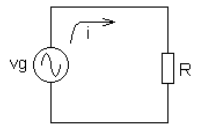
\includegraphics[scale=0.8]{fig1.png}
\end{figure}
La tensión $V_{g}$ tendrá un valor instantáneo que vendrá dado en todo momento por:
$$
V_{g} = V_{0}\sen(2\pi f t)
$$
En corriente alterna la oposición al paso de la corriente eléctrica tiene dos componentes, una real y otra imaginaria. Dicha oposición ya no se llama resistencia sino impedancia, $Z$. La impedancia se expresa mediante un número complejo, por ejemplo de la forma $a+\mathrm{j}b$, siendo $a$ la parte real del número complejo y $b$ su parte imaginaria. Pues bien, una resistencia presenta una impedancia que solo tiene componente real, ya que su componente imaginaria es de valor cero. Tendremos entonces que en el caso que nos ocupa la impedancia total del circuito será igual al valor que presenta la resistencia $R$, ya que no existe ningún otro elemento en el circuito. Así pues:
$$
Z = R + \mathrm{j}0
$$
\section{Circuito C en corriente alterna}
Este tipo de oposición al paso de la corriente eléctrica es de carácter reactivo, entendiendo tal cosa como una ``reacción''  que  introduce  el  condensador  cuando  la  tensión  que  se  le  aplica  tiende  a  variar  lentamente  o  nada. 
\begin{figure}[H]
\centering
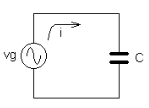
\includegraphics[scale=0.8]{fig2.png}
\end{figure}
Cuando el condensador está totalmente descargado se comporta como un cortocircuito. Cuando está totalmente cargado  como  una  resistencia  de  valor  infinito.  Para  valores  intermedios  de  carga  se  comportará  como  una  resistencia  de  valor  intermedio,  limitando  la  corriente  a  un  determinado  valor.  Como  en  corriente  alterna  el  condensador  está  continuamente  cargándose  y  descargándose,  mientras  más  lentamente  varíe  la  tensión  (frecuencia baja) más tiempo estará el condensador en estado de casi carga que en estado de casi descarga, con lo que  presentará  de  media  una  oposición  alta  al  paso  de  la  corriente.  Para  variaciones  rápidas  de  la  tensión  (frecuencias  altas)  el  efecto  será  el  contrario  y  por  tanto  presentará  una  oposición  baja  al  paso  de  la  corriente.  Podemos  decir,  por  tanto,  que  la  naturaleza  de  este  tipo  de  oposición  es  de  carácter  electrostático:  la  carga  almacenada en el condensador se opone a que éste siga cargándose y esta oposición será mayor cuanto más carga acumule el condensador.
$$
Z = 0 - \mathrm{j}X_{C}
$$
Donde $X_{C}$ es la reactancia capacitiva que se calcula así:
$$
X_{C} = \frac{1}{2\pi f C}
$$
Como puede apreciarse, la impedancia que presenta un condensador solo tiene componente imaginaria reactiva.
\section{Circuito L en corriente alterna}
La  bobina  presentará  oposición  al  paso  de  la  corriente  eléctrica  y  ésta  será  reactiva,  de  manera  similar  al  caso  capacitivo.
\begin{figure}[H]
\centering
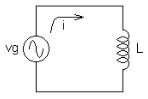
\includegraphics[scale=0.8]{fig3.png}
\end{figure}
Sin  embargo,  la  naturaleza  de  la  reactancia  inductiva  no  es  de  carácter  electrostático,  sino  de  carácter electromagnético. Una bobina inducirá en sus extremos (debido a su autoinducción) una tensión que se opondrá  a  la  tensión  que  se  le  aplique,  al  menos  durante  unos  instantes.  Ello  provoca  que  no  pueda  circular  corriente  libremente.  Cuanto  mayor  sea  la  velocidad  de  variación  de  la  tensión  aplicada  mayor  valor  tendrá  la  tensión  inducida  en  la  bobina  y,  consecuentemente,  menor  corriente  podrá  circular  por  ella.  Así,  a  mayor  frecuencia  de  la  tensión  aplicada  mayor  será  la  reactancia  de  la  bobina  y  a  menor  frecuencia  de  la  tensión  aplicada menor será la reactancia de la bobina.
$$
Z = 0 + \mathrm{j}X_{L}
$$
$$
X_{L} = 2\pi f L
$$
\section{Circuito RLC en corriente alterna}
$$
Z = \frac{1}{\frac{1}{R} - \frac{1}{\mathrm{j}X_{C}} + \frac{1}{\mathrm{j}X_{L}}}
$$
Reemplazando $X_{C}$ y $X_{L}$:
$$
Z = \frac{\mathrm{j}\omega L R}{\mathrm{j}\omega L - \omega^{2}RLC + R}
$$
\chapter{Recomendaciones}
\begin{enumerate}
\item Tener cuidado con las mediciones del multímetro debido a que habrán casos en el que la corriente sea mayor a 5 amperios y esto puede hacer que queme el fusible en el amperímetro si no se ha colocado en la escala adecuada.
\item Se aconseja usar la pinza amperimétrica para una mejor medición y no tener problemas con la escala.
\item Regular muy bien el autotransformador debido a que este voltaje es muy importante en los cálculos.
\item Ser bastante cuidado con la resistencia variable porque no se encuentra en buen estado y generalmente oscila su valor.
\item Cerciorarse del buen funcionamiento de la inductancia.
\item No olvidar agregar en sus cálculos el valor de la resistencia interna de la bobina.
\end{enumerate}
\begin{thebibliography}{99}  %%%este es un contador para el número de bibliografías utilizados.
\addcontentsline{toc}{chapter}{Bibliograf\'{\i}a} %%% Para introducir la bibliografía en el índice.
%\bibitem{Rahman}{Rahman,Aminur y Doe, Hidekazu; ``Ion transfer of tetraalkylammonium cations at an interface between 
%frozen aqueous solution and 1,2-dichloroethane".{\em{Journal of Electroanalytical Chemistry}} {\bfseries 424},159,(1997).}
\bibitem{Gro}{Boylestad, Robert M. ``Introducción al análisis de circuitos''. {\em{Pearson}}}
\bibitem{Gro}{Sadiku, Matthew N. ``Fundamemtos de circuitos eléctricos''. {\em{Mc Graw Hill}}}
%\bibitem{Ding}{Ding, Zhifeng. ``Spectroelectrochemistry and photoelectrochemistry of charge transfer at liquid/liquid
%interfaces". {\em {Tesis, EPFL,}}(1999).}
%\bibitem{AL}{Alonso, Jose M. \em{Técnicas de mecanizado 1}}
%\bibitem{AL}{Alonso, Jose M. ``Técnicas de mecanizado 1". {\em{Paraninfo}} {\bfseries España-Madrid}, 6-20, (2001).}
%\bibitem{Samec2}{Samec Z., Lhotsky A., Jänchenová H., y Marecek, V. ``Interfacial tension and impedance measurements
%of interfaces between two inmiscible electrolyte solutions". {\em{Journal of Electroanalytical Chemistry}} {\bfseries
%43}, 47, (2000).}
%\bibitem{Day}{Day R.A. y Underwood A.L. {\textit{Química Analítica Cuantitativa}},5ºed. Prentice-Hall, México, 1998. 45-48.}
%\bibitem{Keyser}{Farah Abud, Michel. ``Determinación de la vida útil en herramientales de corte endurecido por el proceso de borurización en pasta''. {\em{Instituto tecnológico y de estudios superiores de Monterrey}}}
%\bibitem{Zolotorevski}{Escalona, I. ``Máquinas: herramientas por arranque de viruta.''.{\em{El Cid Editor.}}}
%\bibitem{Lasheras}{Lasheras. ``Tecnología de los Materiales Industriales''.} 
%\bibitem{Dieter}{Dieter. ``Metalurgia mecánica''.}
%\bibitem{Apraiz}{Apraiz, J. ``Tratamiento Térmico de los Aceros''.}
%\bibitem{Smith}{Smith, William F. y Ph.D. Hashemi, Javad ``Ciencia e ingeniería de materiales". {\em{
%Madrid: McGraw-Hill, Interamericana de España.}} 570, (2004).} 
%\bibitem{Callister}{Callister, William D. y Rethwisch, David G. ``Introducción a la ingeniería de los materiales''. %{\em{Barcelona Reverté.}}, 960, (2007).} 
%\bibitem{Askeland}{Askeland, Donald R., Pradeep P. Phulé y Wright, Wendelin J. ``Ciencia e ingeniería de los materiales''.{\em{México, D.F. Internacional Thomson Editores.}} {\textit{$6^{ta}$ edición}}, 1004, (2012).}
%\bibitem{HARDBANDING}{Tabla de conversión de escala de durezas. \begin{verbatim}http://%hardbandingsolutions.com/postle_sp/hardness.php
%\end{verbatim}}
%\bibitem{HE}{Fresadora. \begin{verbatim} http://lizdenbow.blogspot.com/
%\end{verbatim}}
%\bibitem{ASTM}{Normas ASTM.}
%\bibitem{NTP}{Normas NTP.}
\end{thebibliography}
\end{document}